\section{Introduction to Computer Vision}
\begin{frame}{}
    \LARGE Computer Vision: \textbf{Introduction}
\end{frame}

\begin{frame}{Computer Vision}
\centering
Building artificial systems that process, perceive, and reason about visual data
\end{frame}

\begin{frame}{Computer Vision is Everywhere}
\begin{figure}
\centering
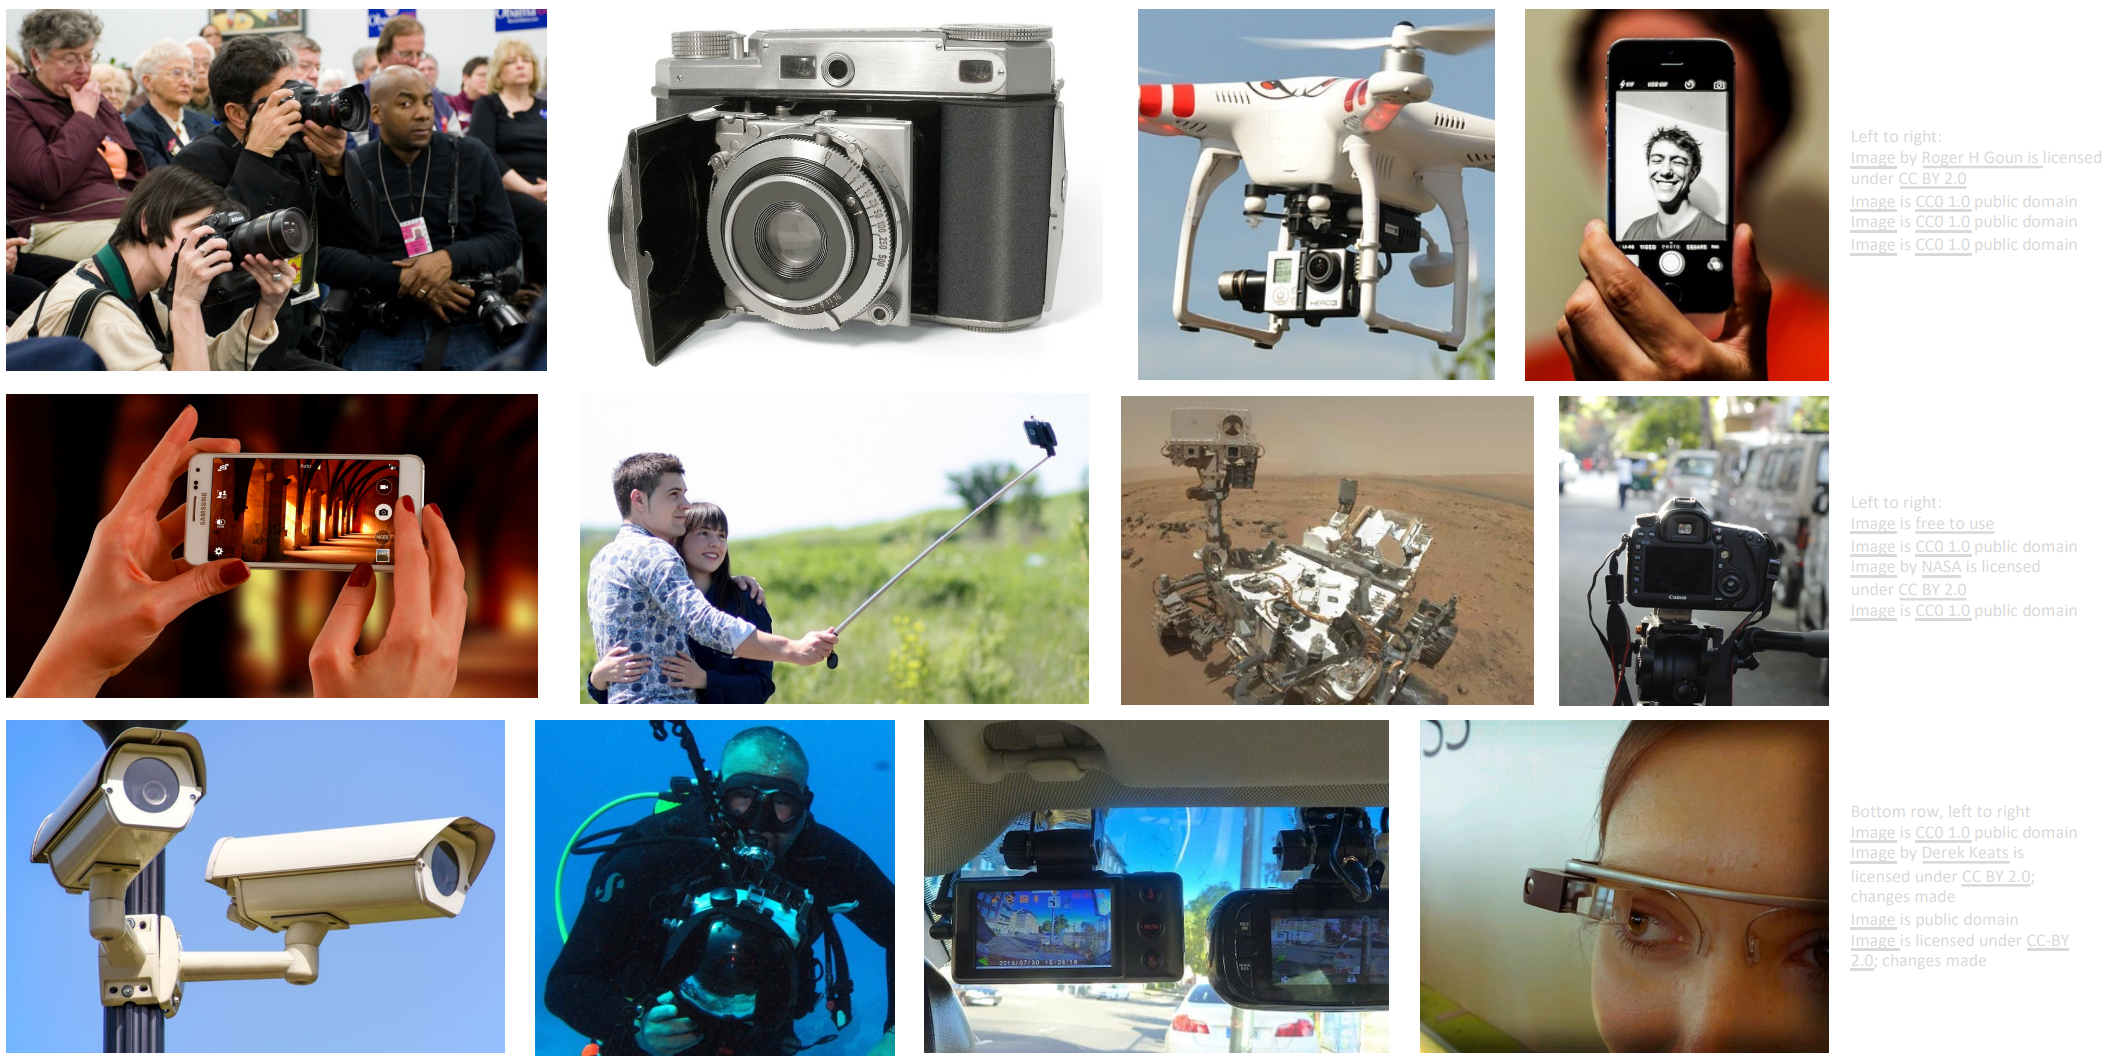
\includegraphics[width=1.0\textwidth,height=1.0\textheight,keepaspectratio]{images/cv-intro/cv_1.png}
\end{figure}
\end{frame}

\begin{frame}[allowframebreaks]{Some Applications}
    \foreach \i in {2,...,13} {
        \begin{figure}
            \centering
            \includegraphics[height=0.9\textheight,width=1\textwidth,keepaspectratio]{images/cnn/cv_\i.png}
        \end{figure}

        \framebreak
    }
\end{frame}

\section{Image Representation}
\begin{frame}{How to represent an image?}
\begin{itemize}
    \item Images are represented as Matrices with elements in $[0,255]$
    \item Grayscale images have one channel.
\end{itemize}
\begin{figure}
\centering
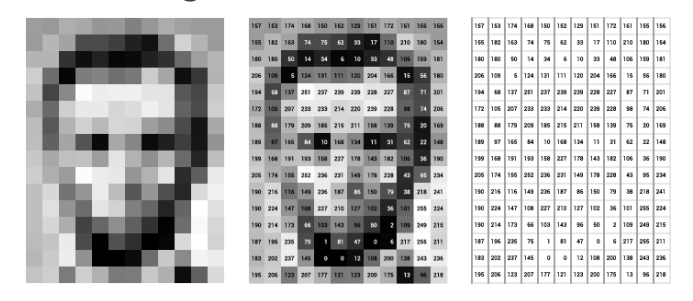
\includegraphics[width=1.0\textwidth,height=0.7\textheight,keepaspectratio]{images/cnn/represent_image.png}
\end{figure}

\footnotetext{https://www.v7labs.com/blog/image-recognition-guide}
\end{frame}

\begin{frame}{How to represent an image?}
\begin{itemize}
    \item RGB images have 3 channels.
\end{itemize}
\begin{figure}
\centering
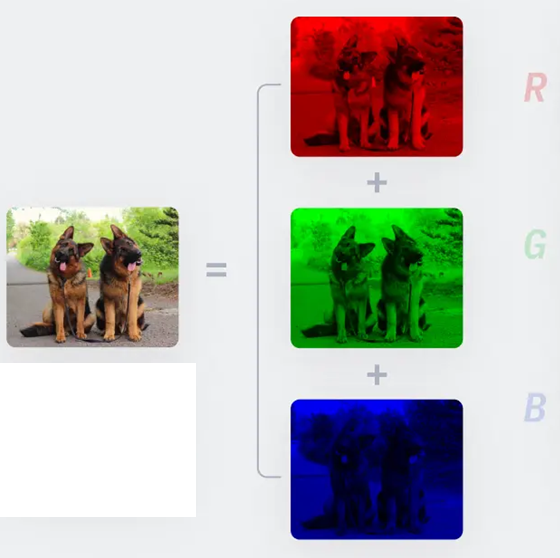
\includegraphics[width=1.5\textwidth,height=0.7\textheight,keepaspectratio]{images/cv-intro/RGB.png}
\end{figure}
\end{frame}
